\section{Hardware-Software Schnittstelle}

\begin{defi}{Transistor}
    \emph{TRANsfer reSISTOR (Transistor)} bedeutet soviel wie \enquote{steuerbarer Widerstand}.

    Im Kontext der Digitaltechnik reicht uns die einfache Vorstellung eines CMOS Transistors als durch Spannung gesteuerte Schalter.
    Sie bestehen aus \texttt{Emitter}, \texttt{Collector} und \texttt{Base}

    \begin{minipage}[t]{0.45\textwidth}
        Der \emph{n-Typ} Transistor schließt, wenn an der Base 3.3V anliegt.

        \begin{center}
            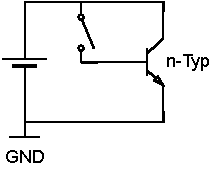
\includegraphics[width=0.5\textwidth]{includes/figures/defi_npn.pdf}
        \end{center}
    \end{minipage}
    \begin{minipage}[t]{0.1\textwidth}
        \
    \end{minipage}
    \begin{minipage}[t]{0.45\textwidth}
        Der \emph{p-Typ} Transistor schließt, wenn an der Base 0V anliegt.

        \begin{center}
            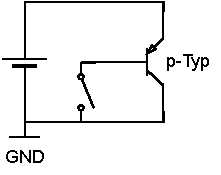
\includegraphics[width=0.5\textwidth]{includes/figures/defi_pnp.pdf}
        \end{center}
    \end{minipage}
\end{defi}

\begin{defi}{Logikgatter mit Transistoren}
    \begin{minipage}[t]{0.33\textwidth}
        \begin{center}
            \emph{NICHT (NOT)}
        \end{center}
    \end{minipage}
    \begin{minipage}[t]{0.33\textwidth}
        \begin{center}
            \emph{UND (AND)}
        \end{center}
    \end{minipage}
    \begin{minipage}[t]{0.33\textwidth}
        \begin{center}
            \emph{ODER (OR)}
        \end{center}
    \end{minipage}

    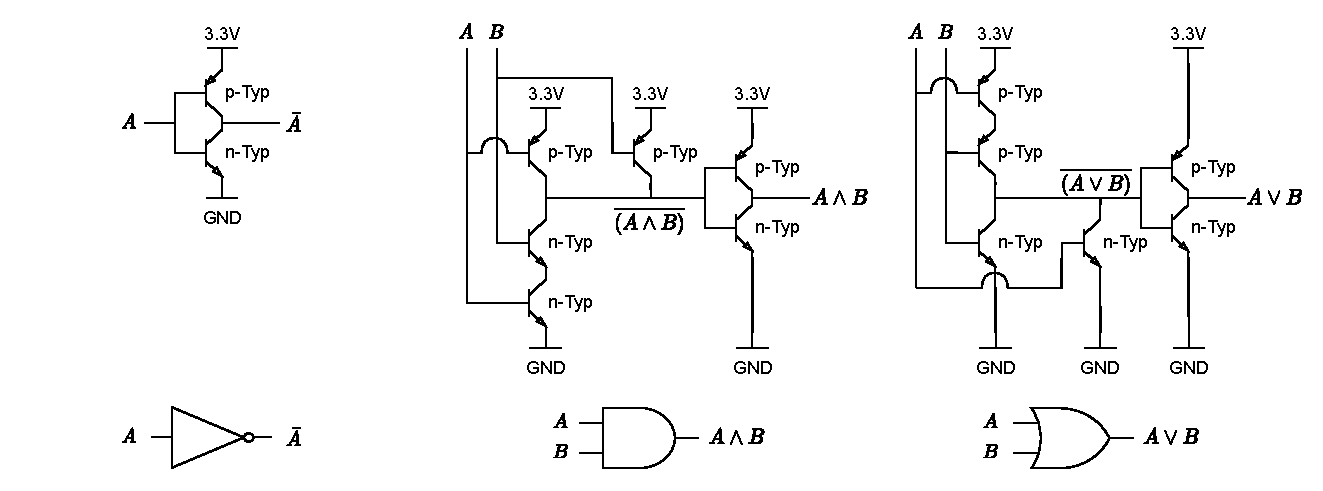
\includegraphics[width=\textwidth]{includes/figures/defi_logikgatter.pdf}

    \begin{minipage}[t]{0.33\textwidth}
        \begin{center}
            \begin{tabular}{|c||c|}
                \hline
                $A$ & $\bar{A}$ \\\hline\hline
                0   & 1         \\\hline
                1   & 0         \\\hline
            \end{tabular}
        \end{center}
    \end{minipage}
    \begin{minipage}[t]{0.33\textwidth}
        \begin{center}
            \begin{tabular}{|c|c||c|}
                \hline
                $A$ & $B$ & $A \land B$ \\\hline\hline
                0   & 0   & 0           \\\hline
                0   & 1   & 0           \\\hline
                1   & 0   & 0           \\\hline
                1   & 1   & 1           \\\hline
            \end{tabular}
        \end{center}
    \end{minipage}
    \begin{minipage}[t]{0.33\textwidth}
        \begin{center}
            \begin{tabular}{|c|c||c|}
                \hline
                $A$ & $B$ & $A \lor B$ \\\hline\hline
                0   & 0   & 0          \\\hline
                0   & 1   & 1          \\\hline
                1   & 0   & 1          \\\hline
                1   & 1   & 1          \\\hline
            \end{tabular}
        \end{center}
    \end{minipage}
\end{defi}

\begin{bonus}{Logikgatter mit Transistoren}
    Da \emph{UND} und \emph{OR} am Ende negiert werden müssen, sind \emph{NAND} und \emph{NOR} \enquote{leichter} zu bauen:

    \begin{center}
        \begin{minipage}[t]{0.33\textwidth}
            \begin{center}
                \emph{NAND}
            \end{center}
        \end{minipage}
        \begin{minipage}[t]{0.33\textwidth}
            \begin{center}
                \emph{NOR}
            \end{center}
        \end{minipage}

        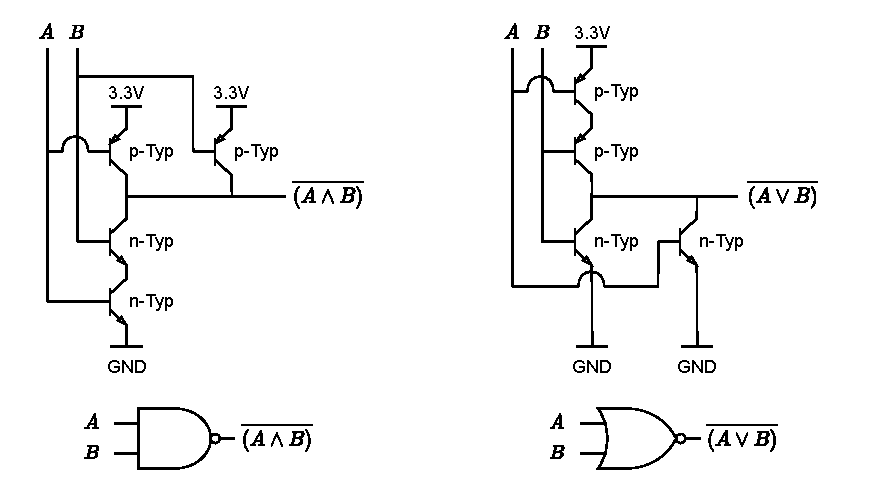
\includegraphics[width=0.66\textwidth]{includes/figures/bonus_logikgatter.pdf}

        \begin{minipage}[t]{0.33\textwidth}
            \begin{center}
                \begin{tabular}{|c|c||c|c|}
                    \hline
                    $A$ & $B$ & $A \land B$ & $\lnot (A \land B)$ \\\hline\hline
                    0   & 0   & 0           & 1                   \\\hline
                    0   & 1   & 0           & 1                   \\\hline
                    1   & 0   & 0           & 1                   \\\hline
                    1   & 1   & 1           & 0                   \\\hline
                \end{tabular}
            \end{center}
        \end{minipage}
        \begin{minipage}[t]{0.33\textwidth}
            \begin{center}
                \begin{tabular}{|c|c||c|c|}
                    \hline
                    $A$ & $B$ & $A \lor B$ & $\lnot (A \lor B)$ \\\hline\hline
                    0   & 0   & 0          & 1                  \\\hline
                    0   & 1   & 1          & 0                  \\\hline
                    1   & 0   & 1          & 0                  \\\hline
                    1   & 1   & 1          & 0                  \\\hline
                \end{tabular}
            \end{center}
        \end{minipage}
    \end{center}
\end{bonus}

\begin{defi}{Treiber}
    \begin{center}
        \emph{Treiber (Three-State Driver)}
    \end{center}

    \begin{minipage}{0.5\textwidth}
        \begin{center}
            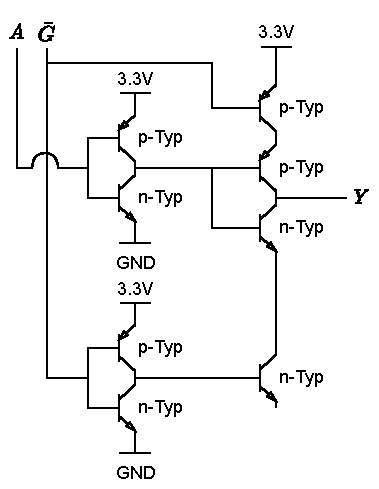
\includegraphics[width=0.66\textwidth]{includes/figures/defi_driver.pdf}
        \end{center}
    \end{minipage}
    \begin{minipage}{0.5\textwidth}
        \begin{center}
            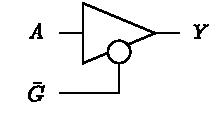
\includegraphics[width=0.4\textwidth]{includes/figures/defi_driver_symbol.pdf}

            \begin{tabular}{|c|c||c|}
                \hline
                $A$ & $\bar{G}$ & $Y$                                                                   \\\hline\hline
                0   & 0         & 0                                                                     \\\hline
                0   & 1         & nc\footnote{\enquote{not connected bzw. dritter hochohmiger Zustand}} \\\hline
                1   & 0         & 1                                                                     \\\hline
                1   & 1         & nc                                                                    \\\hline
            \end{tabular}
        \end{center}
    \end{minipage}
\end{defi}

\begin{defi}{Multiplexer}
    Ein \emph{Multiplexer} wird genutzt um an einen Ausgang mehrere Eingänge anzuschließen, die einzeln weitergeleitet werden.

    \begin{minipage}{0.5\textwidth}
        \begin{center}
            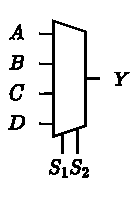
\includegraphics[width=0.3\textwidth]{includes/figures/defi_multiplexer.pdf}
        \end{center}
    \end{minipage}
    \begin{minipage}{0.5\textwidth}
        \begin{center}
            \begin{tabular}{|c|c|c|c|c|c||c|c|}
                \hline
                $A$ & $B$ & $C$ & $D$ & $S_1$ & $S_2$ & $Y$ & $Y$ \\\hline\hline
                0   & *   & *   & *   & 0     & 0     & $A$ & 0   \\\hline
                1   & *   & *   & *   & 0     & 0     & $A$ & 1   \\\hline
                *   & 0   & *   & *   & 0     & 1     & $B$ & 0   \\\hline
                *   & 1   & *   & *   & 0     & 1     & $B$ & 1   \\\hline
                *   & *   & 0   & *   & 1     & 0     & $C$ & 0   \\\hline
                *   & *   & 1   & *   & 1     & 0     & $C$ & 1   \\\hline
                *   & *   & *   & 0   & 1     & 1     & $D$ & 0   \\\hline
                *   & *   & *   & 1   & 1     & 1     & $D$ & 1   \\\hline
            \end{tabular}
        \end{center}
    \end{minipage}
\end{defi}

\begin{defi}{SR-Latch}
    \begin{center}
        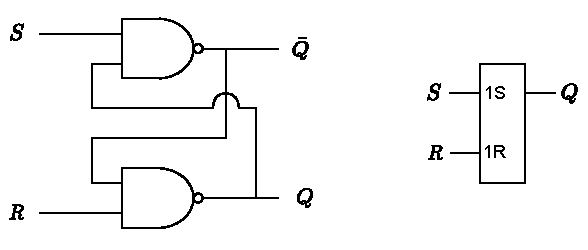
\includegraphics[width=0.5\textwidth]{includes/figures/defi_sr_latch.pdf}
    \end{center}
\end{defi}

\begin{bonus}{SR-Latch Übergänge}
    \begin{center}
        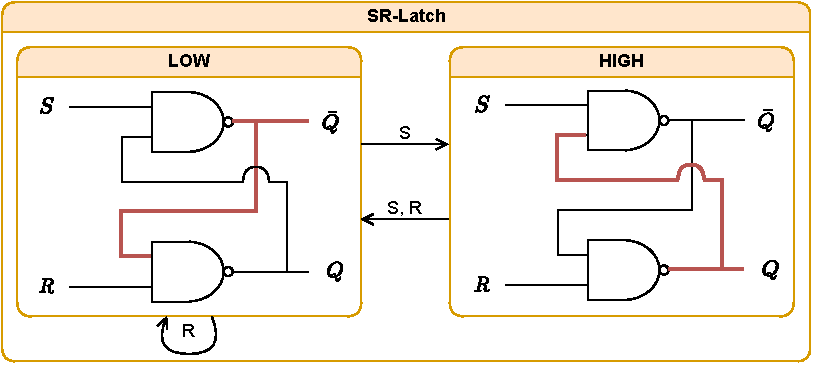
\includegraphics[width=0.75\textwidth]{includes/figures/bonus_sr_latch.pdf}
    \end{center}
\end{bonus}

\begin{defi}{SR-Latch mit Takt}
    Durch die UND-Gatter werden die Set und Reset-Signale nur weitergeleitet, wenn das Clock-Signal HIGH ist.

    \begin{center}
        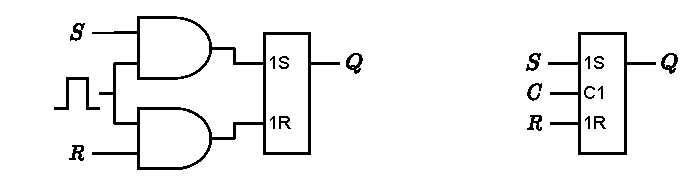
\includegraphics[width=0.75\textwidth]{includes/figures/defi_lr_latch_clock.pdf}
    \end{center}

    Alternativ kann man das Reset Signal mit NOT-Set ersetzen:

    \begin{center}
        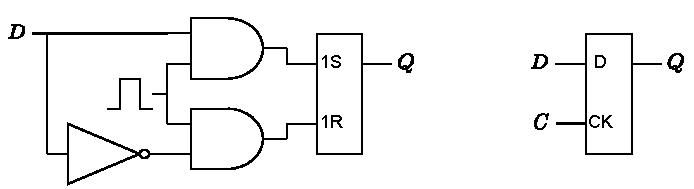
\includegraphics[width=0.75\textwidth]{includes/figures/defi_lr_latch_clock2.pdf}
    \end{center}
\end{defi}

\begin{defi}{Pulsgenerator}
    Häufig soll die Datenübernahme nur bei einer steigenden oder fallenden Flanke des Clock-Signals erfolgen.
    Dazu wird ein Pulsgenerator eingesetzt.

    Sei $\Delta$ die Verzögerung, die die Bauteile zum \enquote{schalten} benötigen:

    \begin{center}
        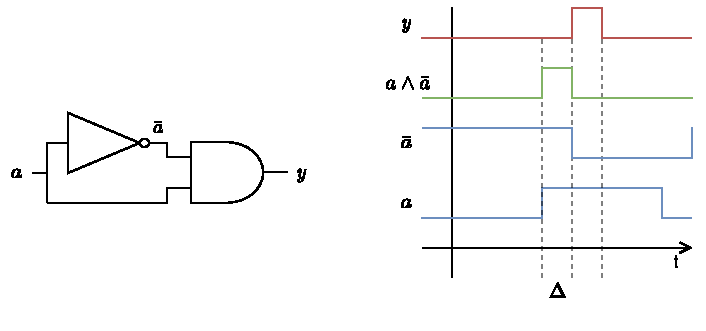
\includegraphics[width=0.75\textwidth]{includes/figures/defi_pulsgenerator.pdf}
    \end{center}
\end{defi}

\begin{defi}{D-Flipflop}
    Ein \emph{D-Flipflop} kombiniert das D-Latch mit einer Flankensteuerung:

    \begin{center}
        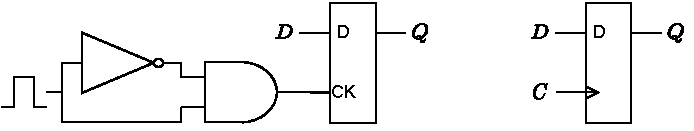
\includegraphics[width=0.75\textwidth]{includes/figures/defi_d_flipflop.pdf}
    \end{center}
\end{defi}

\begin{defi}{MSP432 Speicher Layout}
    ARM Prozessoren besitzen eine Harvard-Architektur.
    Der MSP432 besitzt 32-Bit Adressbusse und 32-Bit Datenbusse.

    Aus der Programmier-Perspektive zeigt jede Adresse jedoch auf einen Byte (8 Bit), nicht ein ganzes 32-Bit Wort.

    Der MSP432 hat einen 4GB Adressraum, der in 512MB-Zonen unterteilt ist:

    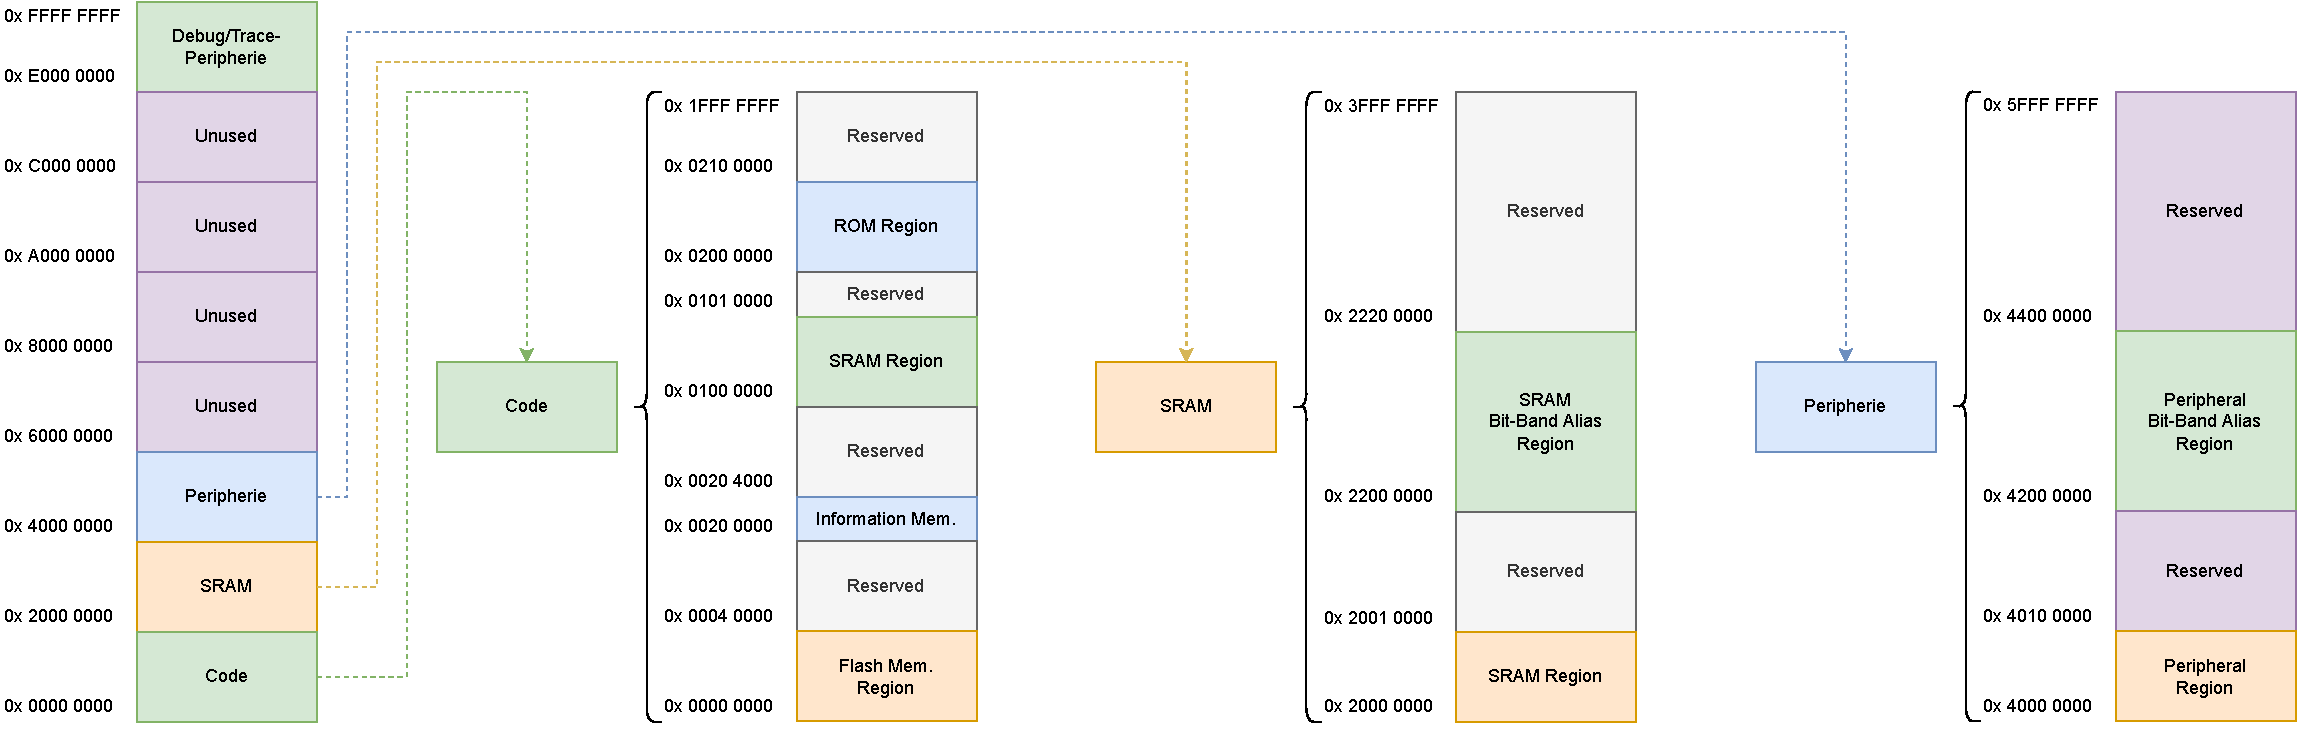
\includegraphics[width=\textwidth]{includes/figures/defi_msp432_speicher.pdf}
\end{defi}

\begin{defi}{GPIO-Register}
    \begin{wrapfigure}{r}{0.35\textwidth}
        \begin{center}
            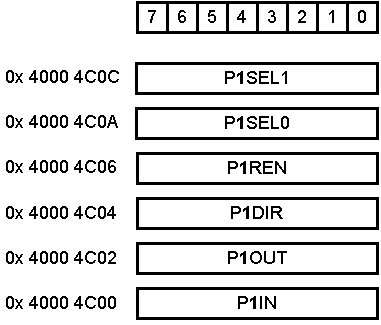
\includegraphics[width=0.3\textwidth]{includes/figures/defi_msp432_port.pdf}
        \end{center}
    \end{wrapfigure}

    Die Einstellungen für einen GPIO Port befinden sich in mehreren Registern.
    Sie sind in folgende Register unterteilt:
    \begin{itemize}
        \item \texttt{SEL1}: Select1
        \item \texttt{SEL2}: Select2
        \item \texttt{REN}: Resistor Enable
        \item \texttt{DIR}: Richtung (Direction)
        \item \texttt{OUT}: Ausgangspegel
        \item \texttt{IN}: Eingangspegel
    \end{itemize}
\end{defi}

\begin{bonus}{Bitmaske}
    Man kann durch die \texttt{msp.h} Bibliothek byteweise auf Register zugreifen.
    Jedoch möchte man anliegende Leitungen nicht beeinflussen.

    Dazu kann man durch logische Verknüpfungen einzelne Bits verändern.

    Sei P1 bis auf das letzte bit (\texttt{$\alpha$}) unbekannt, die Maske für P1.1 \texttt{0000 0001}:

    \begin{center}
        \begin{tabular}{|c|c|c|c|c|}
            \hline
            $\text{P1} \land \text{Maske}$ & $\text{P1} \land \lnot \text{Maske}$ & $\text{P1} \lor \text{Maske}$ & $\text{P1} \lor \lnot \text{Maske}$ & $\text{P1} \oplus \text{Maske}$ \\\hline\hline
            \texttt{0000 0000$\alpha$}     & \texttt{.... ...0}                   & \texttt{.... ...1}            & \texttt{1111 1111$\alpha$}          & \texttt{.... ...$\lnot \alpha$} \\\hline
        \end{tabular}
    \end{center}

    Wir sehen, dass wir um $\alpha$ zu verändern folgende Verknüpfungen nehmen müssen:
    \begin{itemize}
        \item \texttt{0}: $\land \lnot (\text{0000 0001})$
        \item \texttt{1}: $\lor (\text{0000 0001})$
        \item \texttt{$\lnot \alpha$}: $\oplus (\text{0000 0001})$
    \end{itemize}
\end{bonus}

\begin{example}{C Schnittstelle zur Peripherie}
    Wenn wir P1.0\footnote{Auf dem MSP432 die rote LED} als Output setzen wollen, können wir die Register wie folge manipulieren:

    \begin{lstlisting}[language=c]
        #include msp.h

        #define BIT0 (uint16_t) (0x0001) // 0000 0001

        // Select GPIO mode
        P1->SEL0 &= ~BIT0 // .... ...0
        P1->SEL1 &= ~BIT0 // .... ...0

        // Set as output
        P1->DIR |= BIT0   // .... ...1

        // Modify output
        P1->OUT &= ~BIT0  // .... ...0 - Clear P1.0
        P1->OUT |= BIT0   // .... ...1 - Set P1.0
        P1->OUT ^= BIT0   // TOGGLE P1.0
    \end{lstlisting}
\end{example}

\begin{example}{C Schnittstelle zur Peripherie}
    Wenn wir P5.1\footnote{Auf dem MSP432 Schalter 1} als Input setzen wollen, können wir die Register wie folge manipulieren:

    \begin{lstlisting}[language=c]
        #include msp.h

        #define BIT1 (uint16_t) (0x0002) // 0000 0010

        // Select GPIO mode
        P5->SEL0 &= ~BIT1 // .... ...0
        P5->SEL1 &= ~BIT1 // .... ...0

        // Set as input
        P5->DIR &= ~BIT1  // .... ...0

        // Read P5
        P5->IN
    \end{lstlisting}
\end{example}